\chapter{An Alternative View of Belief Propagation}
\label{chapter3}
% set the path to figures in this section
\graphicspath{{source/chapter3/}}

Belief propagation (BP) is a meta message-passing algorithm for inference problems in probabilistic graphical models. BP answers queries by locally exchanging beliefs (statistical information) between nodes in a graphical model \cite{kschischang2001factor_graph, Bishop:2006:PRM:1162264}. In Section~\ref{chpt2:sec:variational-inference}, we introduced the classic belief propagation as the minimization of free energy, instead of an iterative message-passing routine. Interesting to note, the message-passing rule of BP was developed as early as $1986$ \cite{pearl1986b} and had been popularly used in different fields before the free energy optimization intuition was developed in literature \cite{yedidia2003understanding}.

BP can solve inference problems in linear-time exactly when graphs are loop-free or tree-structured \cite{kschischang2001factor_graph}. The message-passing routine of BP can be boiled down into variable elimination in tree-structured graphs\footnote{This applies to cases where systems themselves can be represented by tree-structured graphs, or cases where original graphs are not trees but becoming tree-structured after reorganized (such as clustering).} and message scheduling, which corresponds to determining the variable elimination order. The message scheduling can be omitted and equivalent exact inference results can be obtained, when an alternative belief update algorithm is applied which is also known as Lauritzen-Spiegelhalter algorithm \cite[Section~10.3]{koller2009pgm}. BP and its variants are widely applied in large computation systems due to their 'magic' of reducing the exponential number of operations for inference with enumeration into linear complexity. This is possible because: 
\begin{itemize}
\item An underline distribution of a graphical model is usually factorized, and each sub-expression (a factor) depends only on a small number of variables.
\item The intermediate results are computed once and cached as messages, which are reused in coming computations. 
\end{itemize}

Inevitably, many real-world signals are naturally modeled by graph representations with loops. Surprisingly, although lost its optimality guarantees in loopy graphs, loopy BP is still a practical method and gives reasonable good inference results by running it as if there ware no loops. But its performance can vary from case to case and its behavior is not well understood in general. 

In this chapter, to gain more insights into BP in general graphs, we take a variational approach to develop an interpretable variant of BP, which is termed as $\alpha$-BP.
The intuition of $\alpha$-BP starts with a surrogate distribution $q(\bm{x})$, which is an approximate distribution. $q(\bm{x})$ is assumed to be fully factorized, and each factor of $q(\bm{x})$ actually represents a message in the graphical model with an underlining distribution $p(\bm{x})$. We derive a message-passing rule that is induced by minimizing a localized $\alpha$-divergence. The merits of $\alpha$-BP are as follows: i). {$\alpha$-BP is derived intuitively as localized minimization of $\alpha$-divergence between original distribution $p$ and surrogate distribution $q$}; ii). {$\alpha$-BP generalizes the standard BP, since the message-passing rule of BP is a special case of $\alpha$-BP}. iii). {$\alpha$}-BP can outperform BP in complete (fully-connected) graphs while still maintaining the simplicity of BP for inference.

Apart from the algorithmic perspective, another common issue of BP and its variants in general graphs is convergence. We devote Section~\ref{chpt3:sec:cnvg-thm} to a convergence study of $\alpha$-BP. Sufficient conditions that guarantee the convergence of $\alpha$-BP to a unique fixed point, are studied and obtained. It turns out that the derived convergence conditions of $\alpha$-BP depend on both the graph and also the value of $\alpha$. This result suggests that a proper choice of $\alpha$ can help to guarantee the convergence of $\alpha$-BP.

\section{$\alpha$ Divergence}
\label{chpt3:sec:alpha-divergence}
Before we get into the algorithmic discussion, we firstly provide some preliminaries for the algorithmic intuition. As an extended discussion to Section~\ref{chpt2:sec:devergence}, we firstly introduce a more generalized divergence than $\mathrm{KL}$ divergence.

Apart from the KL divergence, another divergence measure that generalizes KL divergence is $\alpha$-divergence. In fact, $\alpha$-divergence appeared in literature just one year later than KL divergence when Herman Chernoff initially defined it for likelihood-ratio tests \cite{Chernoff1952measure}. Around a decade later, Alfr\'ed R\'enyi proposed his version of divergence as well \cite{renyi1961entropy}. In the 80s of last century, Amari extended Chernoff's version of $\alpha$-divergence \cite{amari1982differential}, which is now widely used in studies of the geometry of distribution manifolds. 
$\alpha$-divergence, similar to KL divergence, is a typical way to measure how different two measures characterized by densities $p$ and $q$ are. By following the notation \cite{Zhu95informationgeometric}, the definition of $\alpha$-divergence (Amari's version, with correction term to accommodate unnormalized measure) is as follows,
\begin{equation}\label{chpt3:eq:alpha-divergence}
  \Dd_{\alpha}(p \| q ) = \frac{\sum_{\bm{x}} \alpha p(\bm{x}) + (1-\alpha) q (\bm{x}) - p(\bm{x})^{\alpha} q(\bm{x})^{1-\alpha}}{\alpha(1-\alpha)},
\end{equation}
where $\alpha$ is the parameter of this divergence. Different from the KL divergence definition in Section~\ref{chpt2:sec:devergence}, $p$ and $q$ here are not necessarily to be normalized measures.

In Section~\ref{chpt2:sec:devergence}, the KL divergence was defined over two normalized measures. Here we extend that definition to a generalized case where $p$ and $q$ are not necessarily normalized, as an extended divergence from the normalized case. As shall be see, KL divergence is closely related with $\alpha$-divergence. KL divergence for general measures is defined as
\begin{equation}\label{chpt3:eq:kl-divergence}
  \mathrm{KL}(p \| q) = \sum_{\bm{x}} p(\bm{x}) \log{\frac{p(\bm{x})}{q(\bm{x})}} + \sum_{\bm{x}} q(\bm{x}) - p(\bm{x}) ,
\end{equation}
where the $\sum_{\bm{x}} q(\bm{x}) - p(\bm{x})$ is a correction factor to accommodate possibly unnormalized $p$ and $q$.
\begin{remark}
  The KL divergence can be seen as a special case of $\alpha$-divergence, by observing $\lim_{\alpha \rightarrow 1}\Dd_{\alpha}(p \| q ) = KL(p\|q)$ and $\lim_{\alpha \rightarrow 0}\Dd_{\alpha}(p \| q ) = KL(q\|p)$ (applying L'H\^opital's rule to \eqref{chpt3:eq:alpha-divergence}).

  Regarding the basic properties of divergence measures, both $\alpha$-divergence and KL divergence are zero when $p=q$, and they are non-negative. 
\end{remark}

Denote the KL-projection by
\begin{equation}
  \text{proj}[p] = \uargmin{q \in \Qq} \mathrm{KL}(p\|q),
\end{equation}
where $\Qq$ is a family of distributions that $q$ belongs to.
According to the stationary point equivalence Theorem in \cite{divergence-measures-and-message-passing}, $\text{proj}[p^{\alpha}q^{1- \alpha}]$ and $\Dd_{\alpha}(p\|q)$ have same stationary points (gradient is zero). This equivalence holds by assuming $\theta$ is parameter of $q(x)$ and observing
\begin{align}
  \pd{\mathrm{KL}(p\|q)}{\theta} &= \sum_{\bm{x}} \pd{q(\bm{x})}{\theta} - \sum_{\bm{x}}\frac{p(\bm{x})}{q(\bm{x})} \pd{q(\bm{x})}{\theta} , \nonumber \\
  \pd{\mathrm{\Dd_{\alpha}}(p\|q)}{\theta} &= \frac{1}{\alpha} \left( \sum_{\bm{x}} \pd{q(\bm{x})}{\theta} - \sum_{\bm{x}}\frac{p^{\prime}(\bm{x})}{q(\bm{x})} \pd{q(\bm{x})}{\theta} \right), \nonumber
\end{align}
with $p^{\prime}(\bm{x}) = p^{\alpha}(\bm{x})q(\bm{x})^{1-\alpha}$. Then it gives $\pd{\mathrm{\Dd_{\alpha}}(p\|q)}{\theta}  = \frac{1}{\alpha}\pd{\mathrm{KL}(p\|q)}{\theta}|_{p=p^{\prime}}$.

A heuristic scheme to find $q^{\ast}$ minimizing $\Dd_{\alpha}(p\|q)$ starts with an initial $q$, and repeatedly updates $q$ via the projection on $\Qq$
\begin{equation}\label{eq:fixed-point-iter}
  q(\bm{x})^{\text{new}}  = \text{proj}[p(\bm{x})^{\alpha}q(\bm{x})^{1-\alpha}].
\end{equation}
This heuristic scheme is a fixed-point iteration, which does not guarantee to converge.

\begin{remark}
  We take $\bm{x}$ to be discrete by default in this section. The sum operation should be replaced by integral for continuous variable $\bm{x}$.
\end{remark}

\section{$\alpha$ Belief Propagation Algorithm}\label{sec:alpha-bp-factor-refine}

\subsection{Pairwise MRF}

\begin{figure}
  \begin{centering}
    \begin{tikzpicture}
      % \tikzstyle{enode} = [thick, draw=blue, circle, inner sep = 3pt,
      % align=center]
      \tikzstyle{enode} = [thick, draw=black, circle, inner sep = 4pt, minimum size = 0.7cm, align=center]
      \tikzstyle{nnode} = [thick, rectangle, rounded corners = 0pt, minimum size = 0.5cm,draw,inner sep = 2pt]

      \tikzstyle{cnode} = [thick, cloud, draw,cloud puffs=10, cloud puff arc=120, aspect=2, inner ysep=4pt]

      \node[cnode] (pajk) at (3, 1.5) {$\Nn(t)\backslash s$};
      \node[cnode] (paik) at (-3, 1.5) {$\Nn(s)\backslash t$};

      \node[nnode] (tk) at (0, 1.5) {};
      \node[] at ($(tk) + (0, 0.5)$) {$\phi_{st}(x_s, x_t)$};
      \node[enode] (xi) at (-1.5 ,0) {};
      \node[] at ($(xi) + (0.75,0)$) {$x_s$};
      
      \node[nnode] (fi) at (-1.5 , -1.5) {};
      \node[] at ($(fi) + (0.95,0)$) {$\phi_s(x_s)$};
      

      \node[enode] (xj) at (1.5 ,0) {};
      \node[] at ($(xj) + (0.75,0)$) {$x_t$};
      
      \node[nnode] (fj) at (1.5 , -1.5) {};
      \node[] at ($(fj) + (0.95,0)$) {$\phi_t(x_t)$};
      
      % connections

      \draw[-] (xi) to (fi);
      \draw[-] (xi) to (tk);
      \draw[-] (xi) to (paik);

      \draw[-] (xj) to (fj);
      \draw[-] (xj) to (tk);
      \draw[-] (xj) to (pajk);
    \end{tikzpicture}
    \vskip -0.1in
    \caption{Factor graph illustration of $p(\bm{x})$ in \eqref{eq:mrf}.}\label{fig:factor-graph}
  \end{centering}
\end{figure}


We consider a probability distribution over random vector $\bm{x} = \left(  x_1, x_2, \cdots,  x_N  \right)$, where $\bm{x} \in \bm{\Xx}$ and $\bm{\Xx}=\prod_{i=1}^N\Xx_i$. For explanation simplicity, we define that each domain is instantiated as the same discrete finite set $\Xx$, i.e., $\bm{\Xx}=\prod_{i=1}^N\Xx$ and $x_i \in \Xx$. Note $\alpha$-BP is applicable for the different domain setting $\bm{\Xx}=\prod_{i=1}^N\Xx_i$. Let us denote the undirected graph of a pairwise MRF by $\Gg:=(\Vv, \Ee)$. $\Vv=\left[ 1 : N \right]$ is the node set associated with the index set of entries of $\bm{x}$. The graph contains undirected edges $\Ee \subset \Vv \times \Vv$, where a pair of $(s, t) \in \Ee$ if and only if nodes $s$ and $t$ are connected by an edge. In addition to the undirected edge set, let us also define the directed edge set induced from $\Gg$ by $\vec{\Ee}$. We have $\abs{\vec{\Ee}} = 2\abs{\Ee}$, where $\abs{\cdot}$ denotes the carnality. These directed edges serve the purpose of convergence analysis only.



The joint distribution of $\bm{x}$ can be formulated as a pairwise factorization form in a pairwise MRF as
\begin{equation}\label{eq:mrf}
  p(\bm{x}) \propto \prod_{{s\in \Vv}} \phi_s(x_s) \prod_{(s,t) \in \Ee} \phi_{st}(x_s, x_t),
\end{equation}
where $\phi_{s}: \Xx \rightarrow (0, \infty)$ and $\phi_{st}: \Xx \times \Xx \rightarrow (0, \infty)$ are factor potentials. Here the normalization is omitted. Note the union of the node set and the edge set, i.e. $\Vv \cup \Ee$, instantiates the factor index set $\Ff$ of a general MRF in \eqref{chp2:eq:mrf-definition} here.

The factor graph representation of \eqref{eq:mrf} is shown in
Figure~\ref{fig:factor-graph}. In the figure, $\Nn(s)$ is the set of variable nodes neighboring $x_s$ via
pairwise factors, i.e. $\Nn(s) = \left\{ t|(t,s) \in \Ee \right\}$, and $\backslash$ denotes exclusion.

\subsection{From $\alpha$-divergence minimization to $\alpha$-BP}
We start with defining a surrogate distribution and then use the surrogate distribution to approximate a given distribution. The message passing rule of $\alpha$-BP is derived by solving the distribution approximation problem.

% \subsubsection{Fully Factorized Surrogate}
We begin with defining a distribution
\begin{equation}
  q(\bm{x}) \propto \prod_{{s\in \Vv}} \tilde{\phi}_s(x_s) \prod_{(s,t) \in \Ee} \tilde{\phi}_{st}(x_s, x_t),
\end{equation}
that is similarly factorized as the joint distribution $p(\bm{x})$. The distribution $q(\bm{x})$ acts as a surrogate distribution of $p(\bm{x})$. The surrogate distribution would be used to estimate inference problems of $p(\bm{x})$. We further choose $q(\bm{x})$ such that it can be fully factorized, which means that $\tilde{\phi}_{s,t}(x_s, x_t)$ can be factorized into product of two independent functions of $x_s, x_t$ respectively. We denote this factorization as
\begin{equation}
  \tilde{\phi}_{s,t}(x_s, x_t) := m_{st}(x_t) m_{ts}(x_s).
\end{equation}
We use the notation $m_{ts}(x_s)$ to denote the factor as a function of $x_s$. $m_{ts}: \Xx \rightarrow (0, \infty)$, serves as the message along directed edge $(t \rightarrow s)$ in our algorithm. Similarly we have factor or message $m_{st}(x_t)$. Then the marginal can be formulated straightforwardly as
\begin{equation}
  q_s(x_s) \propto \tilde{\phi}_s(x_s) \prod_{w\in \Nn(s)} m_{ws}(x_s).
\end{equation}

Now, we are going to use the heuristic scheme as in \eqref{eq:fixed-point-iter} to minimize the information loss by using a fully factorized $q(\bm{x})$ to represent $p(\bm{x})$. The information loss is measured by $\alpha$-divergence $\Dd_{\alpha}(p(\bm{x}) \| q(\bm{x}))$.


We perform a factor-wise refinement procedure to update the factors of $q(\bm{x})$ such that $q(\bm{x})$ approximates $p(\bm{x})$. This approach is similar to the factor-wise refinement procedure in assumed density filtering algorithm\cite{ghosh2016assumed, opper1999bayesian} and expectation propagation \cite{divergence-measures-and-message-passing,Minka:2001:EPA:647235.720257}. Without loss of generality, we begin to refine the factor $\tilde{\phi}_{ts}(x_t, x_s)$ via $\alpha$-divergence with its $\alpha$-parameter assignment as $\alpha_{ts}$. Define $q^{\backslash (t,s)}(\bm{x})$ as the product of all other factors excluding $\tilde{\phi}_{ts}(x_t, x_s)$
\begin{align}
  q^{\backslash (t,s)}(\bm{x})
  = q(\bm{x})/\tilde{\phi}_{ts}(x_t,
  x_s) \propto \prod_{{s\in \Vv}} \tilde{\phi}_s(x_s) \prod_{(v,u) \in
  \Ee\backslash (t,s)}
  \tilde{\phi}_{vu}(x_v, x_u).
  % &= \left(
  %   \tilde{\phi}_s(x_s) \prod_{w\in \Nn(s) \backslash t}m_{ws}(x_s)
  % \right)
  % \left(
  %   \tilde{\phi}_t(x_t) \prod_{w\in \Nn(t) \backslash s}m_{wt}(x_t)
  % \right)
  % \left(
  %   \prod_{v \in \Vv \backslash s,t}
  %   \tilde{\phi}_v(x_v) \prod_{w\in \Nn(v)}m_{wv}(x_v)
  % \right)\nonumber \\
\end{align}
We also exclude the factor $\phi_{ts}(x_t, x_s)$ in $p(\bm{x})$ to obtain $p^{\backslash (t,s)}(\bm{x})$. % Assume that we already have had $q^{\backslash (t,s)}(\bm{x})$ as a good approximation of $p^{\backslash (t,s)}(\bm{x})$, i.e. $q^{\backslash (t,s)}(\bm{x}) \approx p^{\backslash (t,s)}(\bm{x})$, where $\approx$ denotes approximately equality, it is $\tilde{\phi}_{ts}(x_t, x_s)$ that remains to be refined. In refining factor $\tilde{\phi}_{ts}(x_t, x_s)$ with $\alpha$-divergence under such assumption, the problem
Instead of updating $\tilde{\phi}_{ts}(x_t, x_s)$ directly by solving
\begin{equation}
  \!\!\!\uargmin{\tilde{\phi}_{ts}^{\mathrm{new}}(x_t, x_s)}\!\!\!\! \Dd_{\alpha_{ts}}\!\!\left(  p^{\backslash (t,s)}\!(\bm{x})\phi_{ts}(x_t, x_s)\|q^{\backslash (t,s)}\!(\bm{x})\tilde{\phi}_{ts}^{\mathrm{new}}(x_t, x_s)\right),
\end{equation}
we consider the following tractable problem
\begin{equation}\label{eq:alpha-minimize-factor}
  \!\!\!\uargmin{\tilde{\phi}_{ts}^{\mathrm{new}}(x_t, x_s)}\!\!\!\!
  \Dd_{\alpha_{ts}}\!\!\left( q^{\backslash (t,s)}\!(\bm{x}){\phi}_{ts}(x_t, x_s)
    \|q^{\backslash (t,s)}\!(\bm{x})\tilde{\phi}_{ts}^{\mathrm{new}}(x_t, x_s) \right),
\end{equation}
which searches for new factor $\tilde{\phi}_{ts}^{\mathrm{new}}(x_t, x_s)$ such $q$ can approximate $p$ better. In \eqref{eq:alpha-minimize-factor}, $\Dd_{\alpha_{ts}}(\cdot)$ denotes the $\alpha$-divergence with the parameter $\alpha_{ts}$. Note that the approximation \eqref{eq:alpha-minimize-factor} is accurate when $q^{\backslash (t,s)}(\bm{x})$ is equal to $p^{\backslash (t,s)}(\bm{x})$. 
Using fixed-point update in \eqref{eq:fixed-point-iter}, the problem in \eqref{eq:alpha-minimize-factor} is equivalent to
\begin{align}\label{eq:update-rule}
  q^{\backslash (t,s)}(\bm{x})\tilde{\phi}_{ts}^{\mathrm{new}}(x_t, x_s) \propto
  % &\propto \text{proj}\left[ \left( q^{\backslash (t,s)}(\bm{x}){\phi}_{ts}(x_t, x_s) \right)^{\alpha_{ts}} \left(q^{\backslash (t,s)}(\bm{x})\tilde{\phi}_{ts}(x_t, x_s)  \right)^{1-\alpha_{ts}} \right] \nonumber \\
  \mathrm{proj}\left[ q^{\backslash
  (t,s)}(\bm{x}){\phi}_{ts}(x_t, x_s)^{\alpha_{ts}} \tilde{\phi}_{ts}(x_t, x_s)^{1-\alpha_{ts}} \right]. 
\end{align}

Without loss of generality, we update $m_{ts}$ and define
\begin{equation}\label{eq:new_ts}
  \tilde{\phi}_{ts}^{\mathrm{new}}(x_t, x_s) = m_{ts}^{\mathrm{new}}(x_s) m_{st}(x_t).
\end{equation}
Since KL-projection onto a fully factorized distribution reduces to matching the marginals \cite[Proposition~8.3]{koller2009pgm}, substituting \eqref{eq:new_ts} into \eqref{eq:update-rule}, we obtain
\begin{align}\label{eq:message-update}
  \sum_{\bm{x}\backslash x_s} q^{\backslash (t,s)}(\bm{x}) \tilde{\phi}_{ts}^{\mathrm{new}}(x_t, x_s) 
  \propto \sum_{\bm{x}\backslash x_s} q^{\backslash (t,s)}(\bm{x}) \phi_{ts}(x_t, x_s)^{\alpha_{ts}} \tilde{\phi}_{ts}(x_t, x_s)^{1-\alpha_{ts}}.
\end{align}
Solving \eqref{eq:message-update} gives the message passing rule as
\begin{align}\label{eq:message-rule-pairwise}
  {m}^{\text{new}}_{ts}(x_s) \propto  m_{ts}(x_s)^{1-\alpha_{ts}} \bigg[\sum_{x_t} \phi_{ts}(x_t, x_s)^{\alpha_{ts}} {m}_{st}(x_t)^{1-\alpha_{ts}}\tilde{\phi}_t(x_t) \prod_{w\in \Nn(t)\backslash s}m_{wt}(x_t) \bigg].
\end{align}

As for the singleton factor $\tilde{\phi}_t(x_t)$, we can do the refinement procedure on $\tilde{\phi}_t(x_t)$ in the same way as we have done on $\tilde{\phi}_{ts}(x_t, x_s)$. This gives us the update rule of $\tilde{\phi}_t(x_t)$ as
\begin{equation}\label{eq:fix-factor-update}
  \tilde{\phi}_t^{\mathrm{new}}(x_t) \propto \phi_t(x_t)^{\alpha_{t}} \tilde{\phi}_t(x_t)^{1-\alpha_{t}},
\end{equation}
which is the belief from factor $\phi_t(x_t)$ to variable $x_t$. Here $\alpha_t$ is the local assignment of parameter $\alpha$ in $\alpha$-divergence in the refining factor $\tilde{\phi}_t(x_t)$. Note, if we initialize $\tilde{\phi}_t(x_t) = \phi_t(x_t)$, then it remains the same in all iterations, which makes
\begin{align}\label{eq:message-rule}
  {m}^{\mathrm{new}}_{ts}(x_s) \propto
  m_{ts}(x_s)^{1-\alpha_{ts}} \bigg[\sum_{x_t} \phi_{ts}(x_t, x_s)^{\alpha_{ts}} {m}_{st}(x_t)^{1-\alpha_{ts}} {\phi}_t(x_t) \prod_{w\in \Nn(t)\backslash s}m_{wt}(x_t) \bigg].
\end{align}
In our notations, a factor potential is undirected, i.e. $\phi_{ts}(x_t, x_s)=\phi_{st}(x_s, x_t)$ for all $(t,s) \in \Ee$. When refining factors with $\alpha$-BP, each factor potential (corresponding to an edge of $\Gg$) can be associated with a difference setting of $\alpha$ value. In addition we also have $\alpha_{ts} = \alpha_{st}$.

\section{Remarks on $\alpha$ Belief Propagation}\label{subsec:remark}

As discussed in Section~\ref{chpt3:sec:alpha-divergence}, $\mathrm{KL}(p\|q)$ is the special case of $\Dd_{\alpha}(p\|q)$ when $\alpha \rightarrow 1$. When restricting $\alpha_{st}=1$ for all $(s,t) \in \Ee$, the message-passing rule in \eqref{eq:message-rule} becomes
\begin{equation}\label{chpt3:eq:bp-update-rule}
  {m}^{\text{new}}_{ts}(x_s) \propto 
  \sum_{x_t} \phi_{st}(x_s, x_t) {\phi}_t(x_t) \prod_{w\in \Nn(t)\backslash s}m_{wt}(x_t),
\end{equation}
which is exactly the messages of standard BP \cite{Bishop:2006:PRM:1162264}. From this point of view, we can say $\alpha$-BP is a generalization of BP. Additionally, the BP update rule in \eqref{chpt3:eq:bp-update-rule} actually corresponds to the fixed-point iteration assignment by solving the Bethe free energy minimization problem in \eqref{chpt2:bethe-free-energy}.


Note although the mean field method also uses fully-factorized approximation, it is obtained differently from $\alpha$-BP and its factorization differs from that of $\alpha$-BP. From another perspective, mean field methods are actually using information projections from $p(\bm{x})$ to a fully-factorized space via KL divergence as explained in Section~\ref{chpt2:sec:variational-inference}.
In addition, $\alpha$-BP is different from standard BP with damping technique. The latter case uses a message update rule that differs from \eqref{chpt3:eq:bp-update-rule} slightly in the way of assigning updated messages. 


Additionally, $\alpha$-BP differs from the tree-reweighted belief propagation \cite{wainwright2008graphical} in the way of message update rule and also how algorithm is derived. 
The tree-reweighted BP shares some similarity with $\alpha$-BP in the formula of the message-passing rule, namely, the pairwise log-potential functions are scaled by a weight and reweighted old messages appear in the computation of new messages. But different from $\alpha$-BP, tree-reweighted BP is derived by obtaining an upper bound of log-partition function of $p(\bm{x})$ first via a Jensen's inequality and minimize the upper bound. The upper bound is
\begin{align}
  F_T(q) =& \sum_{s\in\Vv}\sum_{x_s}q_s(x_s) \ln{\frac{q_s(x_s)}{\phi_s(x_s)}}  + \sum_{(s,t)\in\Ee}\mu_{st}\sum_{x_s, x_t} q_{st}(x_s, x_t) \ln\frac{q_{st}(x_s,x_t)}{q_s(x_s)q_t(x_t)} \nonumber \\
          & - \sum_{(s,t)\in\Ee}\sum_{x_s, x_t} q_{st}(x_s, x_t)\ln{\phi_{st}(x_t, x_t)},
\end{align}
where $0\leq \mu_{st} \leq 1$ is defined as the appearance probability of edge $(s, t) \in \Ee$, which denotes the appearance rate of edge $(s,t)$ among all spanning trees of graph $\Gg$. Denote the set of all spanning trees of $\Gg$ by $\Tt(\Gg)$. $\mu_{st}$ is the probability that edge $(s,t)$ exists in a randomly selected spanning tree from $\Tt(\Gg)$. The appearance rate can be expensive to compute as it is defined on all spanning trees of a graph.


The upper bound $F_T$ can be reduced into the Bethe free energy \eqref{chpt2:bethe-free-energy} when $\mu_{st}=1$, $\forall ~(s,t)\in \Ee$. The message-passing updates of the tree-reweighted algorithm corresponds to the minimization of $F_T$ with marginalization constraints, which can be written as
\begin{align}
  {m}^{\text{new}}_{ts}(x_s) \propto \sum_{x_t} \phi_{st}(x_s, x_t)^{1/\mu_{st}} {\phi}_t(x_t) \frac{\prod_{w\in \Nn(t)\backslash s}m_{wt}(x_t)^{\mu_{wt}} }{m_{st}(x_t)^{1-\mu_{st}}}.
\end{align}
In the message update rule, both pairwise potential factor and old messages are reweighted, which are different from the way of how pairwise potential factor and old message are reweighted in message update in \eqref{eq:message-rule}. Nevertheless, $\alpha$-BP is derived in a way that is different from tree-reweighted BP.

\begin{figure}[!t]
  \begin{centering}
    \begin{tikzpicture}
      \tikzstyle{enode} = [thick, draw=black, circle, inner sep = 4pt, minimum size = 0.7cm, align=center]
      \tikzstyle{nnode} = [thick, rectangle, rounded corners = 0pt, minimum size = 0.5cm,draw,inner sep = 2pt]

      \tikzstyle{cnode} = [thick, cloud, draw,cloud puffs=10, cloud puff arc=120, aspect=2, inner ysep=4pt]

      \node[cnode] (paik) at (-2, 0) {$\Nn(s)$};
      \node[enode] (xi) at (0 ,0) {};
      \node[] at ($(xi) + (0,0.6)$) {$x_s$};

      \node[nnode] (fi) at (0 , -1.5) {};
      \node[] at ($(fi) + (0.95, 0)$) {$\phi_s(x_s)$};

      \node[nnode] (pi) at (2, 0) {};
      \node[] at ($(pi) + (0, 0.6)$) {$\hat{p}_s(x_s)$};
      % connections
      \draw[-] (xi) to (fi);
      \draw[-] (xi) to (pi);
      \draw[-] (xi) to (paik);
    \end{tikzpicture}
    \caption{Modified graphical model with prior factor.}\label{fig:factor-graph-with-prior}
  \end{centering}
\end{figure}


From the practical perspective, $\alpha$-BP as a meta algorithm can be used with other methods in a hybrid way. Inspired by \cite{pseudo_priorBP2010} and assembling methods \cite{James:2014:ISL:2517747}, we can modify the graphical model shown in Figure~\ref{fig:factor-graph} by adding an extra factor potential $\hat{p}_s(x_s)$ to each $x_s$. The extra factor potential $\hat{p}_s(x_s)$ acts as prior information that can be obtained from other methods. In other words, this factor potential stands for our belief from exterior estimation. Then we can run our $\alpha$-BP on the modified graph. The modified graph is shown in Figure~\ref{fig:factor-graph-with-prior}.

% We summarize the $\alpha$-BP into the pseudo-code in Algorithm~\ref{alg:alphaBP}.

% \begin{algorithm}[tb]
%   \caption{Algorithm of $\alpha$-BP}\label{alg:alphaBP}
%   \begin{algorithmic}
%     \STATE {\bfseries Input:} Graphic model of $p(\bm{x})$
%     \STATE Initialize $q(\bm{x})$
%     \IF {Prior belief on $x_i$ available}
%     \STATE Add prior factor as Figure~\eqref{fig:factor-graph-with-prior}
%     \ENDIF
%     \REPEAT
%     \FOR {each directed edge $(t \rightarrow s)$ of graph model of $p(\bm{x})$}
%     \STATE Message passing by \eqref{eq:message-rule} (or
%     \eqref{eq:message-rule-pairwise}, \eqref{eq:fix-factor-update} if $\tilde{\phi}_s(x_s)$ is not initialized as $\phi_s(x_s)$)
%     \ENDFOR
%     \UNTIL{Converge or maximum number of iteration reached.}
%   \end{algorithmic}
% \end{algorithm}


\section{Convergence of $\alpha$-BP with a Binary State Space}\label{chpt3:sec:cnvg-thm}

As pointed earlier, a key issue of BP and its variants is whether and when they converge. In this section, we discuss when $\alpha$-BP converges. 
From the high-level perspective, we are going to use \textit{contraction} property to show when $\alpha$-BP does converge.
\begin{definition}\label{chpt3:def:contraction}
  For a number $c \in [0,1)$, an operator $G$ over a metric space $(\Delta, d(,))$ is $c$-contraction relative to the distance function $d(,)$ if for any $\bm{z}, \bm{z}^{\prime} \in \Delta$, we have
  \begin{equation}
    d(G(\bm{z}), G(\bm{z}^{\prime})) \leq c d(\bm{z}, \bm{z}^{\prime}).
  \end{equation}
\end{definition}
Definition~\ref{chpt3:def:contraction} tells us that an operator is a contraction if its application to two points in the space is guaranteed to decrease the distance between them by at least a constant $c < 1$. \textit{Thus, we essentially are going to show that the message update rule of $\alpha$-BP is actually a contraction, under which condition we would show that $\alpha$-BP converges}.

We consider the case of binary $\Xx$ with $\Xx=\left\{ -1, 1 \right\}$, to gain insights into the convergence behavior of $\alpha$-BP. The factor potentials are further detailed as
\begin{align}
  \phi_{st}(x_s, x_t) &= \exp\left\{ \theta_{st}(x_s, x_t)\right\}, \nonumber \\
  \phi_{s}(x_s) &= \exp\left\{ \theta_{s}(x_s) \right\}.
\end{align}
Further assume the symmetric property of potentials
\begin{align}\label{chpt3:eq:symmetric-prop}
  \theta_{ts}(x_t, x_s) &= -\theta_{ts}(x_t, -x_s) = -\theta_{ts}(-x_t, x_s), \nonumber\\
  \theta_{s}(x_s) &= - \theta_s(-x_s).
\end{align}

\begin{example}
  The Ising model, from statistical physics \cite{ising1925, PhysRev.65.117}, is such a model whose potentials fulfill the symmetric property in \eqref{chpt3:eq:symmetric-prop}. In the graph $\Gg = (\Vv, \Ee)$ of an Ising model, the random variable $x_s$ takes the spin value $\left\{ $-1$, $+1$ \right\}$. The values of $\bm{x}$ associated with the nodes of $\Gg$ might represent the orientations of magnets in a field or the states of particles of gas in the context of statistical physics. Two elements $x_t$ and $x_s$ of $\bm{x}$ are allowed to interact directly only if there is an edge between them directly, i.e., $(t, s) \in \Ee$. The potential factors of an Ising model is in exponential family. This leads the joint distribution
  \begin{equation*}
    p(\bm{x};\bm{\theta}) \propto \exp\left\{ \sum_{s\in \Vv} b_s x_s + \sum_{(t, s) \in \Ee} J_{ts} x_t x_s \right\},
  \end{equation*}
  the factors of which fulfill the symmetric property in \eqref{chpt3:eq:symmetric-prop}. \textcolor{blue}{an example that fulfills this property, exponential family or coding stuff (check with Ragnar)}
\end{example}

For notation simplicity, we use $\theta_{ts}=\theta_{ts}(1, 1)$ and $\theta_s = \theta_s(1)$. Denote by $\bm{\alpha}$ the vector of all local assignments of parameter $\alpha$, i.e. $\bm{\alpha} = \left(  \alpha_{ts} \right)_{(t ,s) \in \Ee }$, by $\bm{\theta}$ the vector of all parameters of the potentials, i.e. $\bm{\theta} = \left(  \theta_{ts} \right)_{(t ,s) \in \Ee }$.  Define a matrix $\bm{M}(\bm{\alpha}, \bm{\theta})$ of size $\abs{\vec{\Ee}} \times \abs{\vec{\Ee}}$, in which its entries are indexed by directed edges $(t\rightarrow s)$, as
\begin{align}\label{eq:matrix_m}
  M_{(t\rightarrow s), (u \rightarrow v)} =
  \begin{cases}
    \abs{ 1 - \alpha_{ts}}, &\quad u=t, v=s, \\
    \abs{ 1 - \alpha_{ts}} \tanh \abs{\alpha_{ts} \theta_{ts}}, & \quad u = s, v =t, \\
    \tanh\abs{\alpha_{ts} \theta_{ts}}, & \quad u \in \Nn(t)\backslash s, v = t, \\
    0, & \quad \mathrm{otherwise}.
  \end{cases}
\end{align}
\begin{theorem}\label{thm:normd}
  For an arbitrary pairwise Markov random field over binary variables,
  if the largest singular value of matrix $\bm{M}(\bm{\alpha}, \bm{\theta})$ is less than one,
  $\alpha$-BP converges to a fixed point. The associated fixed point is unique.
\end{theorem}

\begin{proof}
  Let us define $z_{ts}$ as the log ratio of belief from node $t$ to node $s$ on two states of $\Xx$, i.e.
  \begin{equation}\label{eq:log-ratio-uv}
    z_{ts} = \log\frac{m_{ts}(1)}{m_{ts}(-1)}.
  \end{equation}

  By combining the local message passing rule in \eqref{eq:message-rule} with \eqref{eq:log-ratio-uv}, we obtain a local update function $F_{ts}: \; \RR^{\abs{\vec{\Ee}}} \rightarrow \RR$ that maps $\bm{z} = \left( z_{ts} \right)_{(t \rightarrow s) \in \Ee}$ to updated $z_{ts}$, which can be expressed as
  % Substituting \eqref{eq:message-rule} into \eqref{eq:log-ratio-uv} gives
  % \begin{align}
      %       &F_{ts}(\bm{z}) = (1- \alpha_{ts})z_{ts} + \\
      %               &\log\frac{\exp\left\{ \alpha_{ts}\left[ \theta_{ts}(1,1) - \theta_{ts}(-1,1) \right] + \theta_t(1) - \theta_t(-1) + (1 - \alpha_{ts})z_{st} + \sum_{w\in \Nn(t)\backslash s} z_{wt} \right\}+1}
                        %                         {\exp\left\{ \alpha_{ts}\left[ \theta_{ts}(1,-1) - \theta_{ts}(-1,1) \right] + \theta_t(1) - \theta_t(-1) + (1 - \alpha_{ts})z_{st} + \sum_{w\in \Nn(t)\backslash s} z_{wt} \right\} +
                        %                         \exp\left\{ \alpha_{ts}\left[ \theta_{ts}(-1,-1) - \theta_{ts}(-1,1) \right] \right\}},
                        %     \end{align}
                        %                         where $\bm{z}$ is vector with element entry $z_{vu}, v,u \in \Vv$.
                        %                         With the symmetric property, the log ratio updates for $z_{ts}$ can be reduced as
  \begin{equation}\label{eq:ratio-update}
    F_{ts}(\bm{z}) = (1-\alpha_{ts}) z_{ts} + f_{ts}(\bm{z}),
  \end{equation}
  where
  \begin{equation}
    f_{ts}(\bm{z}) = \log\frac{\exp\left\{ 2 \alpha_{ts} \theta_{ts} + \Delta_{ts}(\bm{z}) \right\}+1}
    {\exp\left\{ \Delta_{ts}(\bm{z}) \right\} +
      \exp\left\{ 2 \alpha_{ts} \theta_{ts} \right\}},
  \end{equation}
  with
  \begin{equation}
    \Delta_{ts}(\bm{z}) = 2 \theta_s + (1 - \alpha_{ts}) z_{st} + \sum_{w\in \Nn(u)\backslash t} z_{wt}.
  \end{equation}

  In the following, we use superscript ${(n)}$ to denote the $n$-th iteration. Since $f_{ts}$ is continuous on $\RR^{\abs{\vec{\Ee}}}$ and differentiable, we have
  \begin{align}\label{eq:ratio_diff_at_n}
    & z_{ts}^{(n+1)} - z_{ts}^{(n)} \nonumber \\
    =& (1-\alpha_{ts}) (z_{ts}^{(n)} - z_{ts}^{(n-1)}) + f_{ts}(\bm{z}^{(n)}) - f_{ts}(\bm{z}^{(n-1)}) \nonumber \\
    \overset{(a)}{=}& (1-\alpha_{ts}) (z_{ts}^{(n)} - z_{ts}^{(n-1)}) + \nabla f_{ts}(\bm{z}^{\lambda})^{T} (\bm{z}^{(n)} - \bm{z}^{(n-1)}),
  \end{align}
  where $(a)$ follows by the mean-value theorem, $\bm{z}^{\lambda} = \lambda \bm{z}^{(n)} + (1 - \lambda) \bm{z}^{(n-1)}$ for some $\lambda \in (0,1)$, and $\nabla f_{ts}(\bm{z}^{\lambda})$ denotes the gradient of $f_{ts}$ evaluated at $\bm{z}^{\lambda}$. In further details, $\nabla f_{ts}$ is given by
  \begin{equation}\label{eq:F_pd}
    \pd{f_{ts}}{z}=
    \begin{cases}
      ( 1 - \alpha_{ts}) \pd{f_{ts}}{\Delta_{ts}}, &\quad z = z_{st}, \\
      \pd{f_{ts}}{\Delta_{ts}}, &\quad z = z_{wt}, w\in N(t)\backslash s. \\
      0, &\quad \mathrm{otherwise}.  \\
    \end{cases}
  \end{equation}
  
  Our target here is to find the condition to make sequence $\left( z_{ts}^{(n+1)} - z_{ts}^{(n)} \right)$ to converge. To this aim we need to bound the term $\nabla f_{ts}(\bm{z}^{\lambda})^{T} (\bm{z}^{(n)} - \bm{z}^{(n-1)})$ in \eqref{eq:ratio_diff_at_n}. For this purpose, we need two auxiliary functions $H, G: \RR^2 \rightarrow \RR$ from Lemma~$4$ in \cite{roosta2008reweighed_sum_product}, which are given in the following for completeness,
  \begin{align}
    H(\mu; \kappa) &:= \log \frac{\exp(\mu + \kappa) +1}{\exp(\mu) + \exp(\kappa)}, \nonumber \\
    G(\mu; \kappa) &:= \frac{\exp(\mu + \kappa)}{\exp(\mu + \kappa) + 1} - \frac{\exp(\mu)}{\exp(\mu) + \exp(\kappa)} \nonumber \\
                   &= \frac{\sinh{\kappa}}{\cosh{\kappa} + \cosh{\mu}},
  \end{align}
  where it holds that $\pd{H(\mu; \kappa)}{\mu} = G(\mu; \kappa)$. Further, it holds that
  $\abs{G(\mu; \kappa)} \leq \abs{G(0, \kappa)} = \tanh(\abs{\kappa}/2)$.
  Then we have
  \begin{align}\label{eq:eqv_aux_functions}
    f_{ts}(z) &= H(\Delta_{ts}(\bm{z}) ;2 \alpha_{ts} \theta_{ts}), \nonumber \\
    \pd{f_{ts}}{\Delta_{ts}} &= G(\Delta_{ts}(\bm{z}) ;2 \alpha_{ts} \theta_{ts}),
  \end{align}
  which implies
  \begin{equation}\label{eq:f-bound}
    \bigg|{\pd{f_{ts}}{\Delta_{ts}}}\bigg| \leq \tanh(\abs{\alpha_{ts}\theta_{ts}}).
  \end{equation}
  Combining \eqref{eq:ratio_diff_at_n}, \eqref{eq:F_pd}, \eqref{eq:eqv_aux_functions} and \eqref{eq:f-bound}, we have
  \begin{align}\label{eq:ratio_cvg_step}
    &\abs{z_{ts}^{(n+1)} - z_{ts}^{(n)}} \nonumber\\
    & = \abs{(1-\alpha_{ts}) (z_{ts}^{(n)} - z_{ts}^{(n-1)}) + \nabla f_{ts}(\bm{z}^{\lambda})^{T} (\bm{z}^{(n)} - \bm{z}^{(n-1)})} \nonumber \\
    & \leq \abs{(1-\alpha_{ts}) (z_{ts}^{(n)} - z_{ts}^{(n-1)})} + \abs{\nabla f_{ts}(\bm{z}^{\lambda})^{T} (\bm{z}^{(n)} - \bm{z}^{(n-1)})} \nonumber \\
    & = \abs{ 1 - \alpha_{ts}} \abs{z_{ts}^{(n)} - z_{ts}^{(n-1)}} + \abs{\nabla f_{ts}(\bm{z}^{\lambda})}^{T} \abs{\bm{z}^{(n)} - \bm{z}^{(n-1)}} \nonumber \\
    & \overset{(a)}{\leq} \abs{ 1 - \alpha_{ts}} \abs{z_{ts}^{(n)} - z_{ts}^{(n-1)}} + \abs{ 1 - \alpha_{ts}} \tanh(\abs{\alpha_{ts} \theta_{ts}}) \abs{z_{st}^{(n)} - z_{st}^{(n-1)}} \nonumber \\
    &+ \sum_{w\in N(t)\backslash s} \tanh(\abs{\alpha_{ts} \theta_{ts}}) \abs{z_{wt}^{(n)} - z_{wt}^{(n-1)}},
  \end{align}
  where step $(a)$ holds by applying \eqref{eq:F_pd} and \eqref{eq:f-bound}.

  
  Concatenating all $(t\rightarrow s) \in \vec{\Ee}$ for inequality \eqref{eq:ratio_cvg_step} gives
  \begin{equation}\label{eq:ratio-update-ineq}
    \abs{\bm{z}^{(n+1)} - \bm{z}^{n}} \leq \bm{M}(\alpha, \bm{\theta})\abs{\bm{z}^{(n)} - \bm{z}^{n-1}},
  \end{equation}
  where $\bm{M}(\bm{\alpha}, \bm{\theta})$ is defined in \eqref{eq:matrix_m}, and $\leq$ in \eqref{eq:ratio-update-ineq} denotes the element-wise inequality. Also note that in \eqref{eq:ratio-update-ineq}, the $\abs{\cdot}$ operator on a vector is a bit abused and denotes the element-wise absolute operation on the vector. From \eqref{eq:ratio-update-ineq}, we could further have
  \begin{align}\label{eq:ine-normp-iteration}
    \norm{\bm{z}^{(n+1)} - \bm{z}^{n}}_{p} &\leq \norm{\bm{M}(\alpha, \bm{\theta})(\bm{z}^{(n)} - \bm{z}^{n-1})}_{p},               
  \end{align}
  where $1\leq p < \infty$, and $\norm{\cdot}_p$ denotes the ${\ell}^p$-norm.

  When applying $p=2$ to \eqref{eq:ine-normp-iteration}, we have
  \begin{align}\label{eq:ieq-largest-singular}
    \normd{\bm{z}^{(n+1)} - \bm{z}^{(n)}} &\leq \normd{\bm{M}(\bm{\alpha}, \bm{\theta})(\bm{z}^{(n)} - \bm{z}^{(n-1)})} \nonumber \\
                                          &\leq \lambda^{\ast}(\bm{M})\normd{\bm{z}^{(n)} - \bm{z}^{(n-1)}},
  \end{align}
  where $\lambda^{\ast}(\bm{M})$ denotes the largest singular value of matrix
  $\bm{M}(\bm{\alpha}, \bm{\theta})$. If the largest singular value of $\bm{M}$ is less than $1$, the sequence
  $\left( \abs{\bm{z}^{(n+1)} - \bm{z}^{(n)}}\right)$ converges to zero in $\ell^2$-norm as $n \rightarrow \infty$. Therefore, for $\lambda^{\ast}(\bm{M})<1$, $\ell^2$-norm $\left(  \bm{z}^{(n)}  \right)$ is a Cauchy sequence and must converge. 

  By concatenating local update function \eqref{eq:ratio-update}, we have a global update function $\bm{F} = \left(  F_{ts}  \right)_{ (t \rightarrow s) \in \vec{\Ee}}$, which defines a mapping from $\RR^{\abs{\vec{\Ee}}}$ to $\RR^{\abs{\vec{\Ee}}}$. $\bm{F}$ is a continuous function of $\bm{z}$, and we have
  \begin{equation}
    \bm{F}(\lim_{n\rightarrow \infty}\bm{z}^{(n)}) = \lim_{n\rightarrow \infty}\bm{F}(\bm{z}^{(n)}).
  \end{equation}
  Assume that $\left(  \bm{z}^{(n)} \right)$ converges to
  $\bm{z}^{\ast}$. Then
  \begin{align}
    \bm{F}(\bm{z}^{\ast}) - \bm{z}^{\ast}
    &= \lim_{n\rightarrow \infty} \bm{F}(\bm{z}^{(n)}) -\lim_{n\rightarrow
      \infty} \bm{z}^{(n)} \nonumber \\
    &= \lim_{n\rightarrow \infty} (\bm{z}^{(n+1)} - \bm{z}^{(n)}) \nonumber \\
    &= 0.
  \end{align}
  Thus $\bm{z}^{\ast}$ must be a fixed point.

  In what follows we show that the fixed point is unique when $\lambda^{\ast}(\bm{M})<1$. Assume that there are two fixed points $\bm{z}_0^{\ast}$ and $\bm{z}_1^{\ast}$ for sequence $\left\{ \bm{z}^{(n)} \right\}$. Then we have
  \begin{align}\label{eq:two-fix-point}
    \bm{F}(\bm{z}_0^{\ast}) &= \bm{z}_0^{\ast}, \nonumber\\
    \bm{F}(\bm{z}_1^{\ast}) &= \bm{z}_1^{\ast}. 
  \end{align}
  Applying \eqref{eq:ieq-largest-singular} gives
  \begin{equation}\label{eq:two-fix-ineq}
    \normd{\bm{F}(\bm{z}_0^{\ast}) - \bm{F}(\bm{z}_1^{\ast})} \leq
    \lambda^{\ast}(\bm{M})\normd{\bm{z}_0^{\ast} - \bm{z}_1^{\ast}}.
  \end{equation}
  Substituting \eqref{eq:two-fix-point} into \eqref{eq:two-fix-ineq}
  gives
  \begin{equation}
    \normd{\bm{z}_0^{\ast} - \bm{z}_1^{\ast}} \leq
    \lambda^{\ast}(\bm{M})\normd{\bm{z}_0^{\ast} - \bm{z}_1^{\ast}},
  \end{equation}
  which gives us $\bm{z}_0^{\ast} = \bm{z}_1^{\ast}$ for $\lambda^{\ast}(\bm{M})<1$ and completes the uniqueness of the fixed point.
\end{proof}

\begin{remark}
  From Theorem~\ref{thm:normd} we can see that the sufficient condition for convergence of $\alpha$-BP is $\lambda^{\ast}(\bm{M}(\bm{\alpha}, \bm{\theta})) < 1$. It is interesting to notice that $\lambda^{\ast}(\bm{M}(\bm{\alpha}, \bm{\theta}))$ is a function of $\bm{\alpha}$ from $\alpha$-divergence and $\bm{\theta}$ from joint distribution $p(\bm{x})$. This means that whether $\alpha$-BP can converge depends on the graph $\Gg= (\Vv, \Ee)$ representing the problem $p(\bm{x})$ and also the choice of $\bm{\alpha}$. Therefore, proper choice of $\bm{\alpha}$ can guarantee the convergence of $\alpha$-BP if the sufficient condition can possibly be achieved for given $\bm{\theta}$.
\end{remark}

\begin{remark}
  \textcolor{blue}{discussion on the quality of the fix point}
  The condition in Theorem~\ref{thm:normd} tells if $\alpha$-BP converges to a fixed point. However, it does not guarantee if the converged fixed point is a global optimum. Error analysis of BP and its variant is a challenging task. We discussed that the exact inference of BP in tree-structured graphs in Section~\ref{chpt2:sec:inference-mp}. The global optimum of loopy BP algorithm can be guaranteed in rare cares, e.g., a ferromagnetic Ising model in which neighbors prefer to be in aligned states\cite{frederic2019fast}.
\end{remark}

Given the fact that $\alpha$-BP would converge if the condition in Theorem~\ref{thm:normd} is fulfilled, the largest singular value computation for large-sized graph could be nontrivial. We give alternative sufficient conditions for the convergence of $\alpha$-BP.

\begin{corollary}\label{chpt3:cor:converge}
  $\alpha$-BP converges to a fixed point if the condition
  \begin{align}\label{chpt3:cor:choose-col}
    \umax{u \rightarrow v}  \abs{1-\alpha_{uv}} + \abs{1-\alpha_{vu}}\tanh{(\abs{\alpha_{vu} \theta_{vu}})} + \sum_{w \in \Nn(v) \backslash u} \tanh{(\abs{\alpha_{{vw}} \theta_{vw}})} < 1,
  \end{align}
  is fulfilled or the condition
  \begin{align}\label{chpt3:cor:choose-row}
    \umax{t \rightarrow s} \abs{1-\alpha_{ts}} (1 + \tanh(\abs{\alpha_{ts} \theta_{ts}})) + (\abs{\Nn(t)}-1)\tanh(\abs{\alpha_{ts} \theta_{ts}}) < 1.
  \end{align}
  is satisfied, where $\abs{\Nn(t)}$ denotes the carnality of the set $\Nn(t)$. The associated fixed point is unique.
\end{corollary}

\begin{proof}
  Setting $p=1$ to \eqref{eq:ine-normp-iteration}, we have
  \begin{equation}
    \normu{\bm{z}^{(n+1)} - \bm{z}^{n}} \leq \normu{\bm{M}(\alpha, \bm{\theta})(\bm{z}^{(n)} - \bm{z}^{n-1})}.
  \end{equation}
  Furthermore, from \eqref{eq:ine-normp-iteration}, we also have
  \begin{equation}
    \normi{\bm{z}^{(n+1)} - \bm{z}^{n}} \leq \normi{\bm{M}(\alpha, \bm{\theta})(\bm{z}^{(n)} - \bm{z}^{n-1})},
  \end{equation}
  where $\norm{\cdot}_{\infty}$ denotes the $\ell^{\infty}$-norm.
  Then we have
  \begin{align}\label{eq:row-col-norm-ineq}
    \normu{\bm{z}^{(n+1)} - \bm{z}^{n}} &\leq \normu{\bm{M}}\normu{(\bm{z}^{(n)} - \bm{z}^{n-1})}, \nonumber \\
    \normi{\bm{z}^{(n+1)} - \bm{z}^{n}} &\leq \normi{\bm{M}}\normi{(\bm{z}^{(n)} - \bm{z}^{n-1})},
  \end{align}
  where we omit the parameters of $\bm{M}$ here for simplicity. We can expand the first multiplicand on the right hand side of \eqref{eq:row-col-norm-ineq} as follows
  \begin{align}
    \normu{\bm{M}} =& \umax{u \rightarrow v}{\sum_{t\rightarrow s} M_{(t\rightarrow s), (u\rightarrow v)}} \nonumber \\
    =& \umax{u \rightarrow v}\abs{1-\alpha_{uv}} + \abs{1-\alpha_{vu}}\tanh{\abs{\alpha_{vu} \theta_{vu}}} + \sum_{w\in \Nn(v) \backslash u} \tanh{\abs{\alpha_{{vw}} \theta_{vw}}}, \nonumber \\
    \normi{\bm{M}} =& \umax{t \rightarrow s}{\sum_{u\rightarrow v} M_{(t\rightarrow s), (u\rightarrow v)}} \nonumber \\
    =& \umax{t \rightarrow s} \abs{1-\alpha_{ts}} (1 + \tanh\abs{\alpha_{ts} \theta_{ts}}) + (\abs{\Nn(t)}-1)\tanh\abs{\alpha_{ts} \theta_{ts}}.
  \end{align}
  When condition $\normu{\bm{M}} < 1$ is met, sequence $\left( \abs{\bm{z}^{(n+1)} - \bm{z}^{n}} \right)$ approaches to zero as $n\rightarrow \infty$. Similarly, condition $\normi{\bm{M}}<1$ can also guarantee the convergence to zero of sequence $\left( \abs{\bm{z}^{(n+1)} - \bm{z}^{n}} \right)$. The analysis for uniqueness of converged fixed point is similar to that in proof of Theorem~\ref{thm:normd}.
\end{proof}
\begin{remark}[\textcolor{blue}{Interpretation to the Results}]
  
  Both Theorem~\ref{thm:normd} and Corollary~\ref{chpt3:cor:converge} offer sufficient conditions for convergence of $\alpha$-BP to a unique fixed point. The obtained results allow us to check if applying $\alpha$-BP in a certain configuration guarantees convergence without running the algorithm practically to try out, which saves computation resources when problems are at scales. To test the fulfillment of the conditions, the first step it to convert a problem to be solved into its pairwise MRF representation $\Gg(\Vv, \Ee)$. Secondly, construct the matrix $\bm{M}$ according to \eqref{eq:matrix_m}. Note the undirected edge set $\Ee$ of $\Gg$ is used to construct a directed edge set $\vec{\Ee}$ by assigning $(s\rightarrow t)$ and $(t\rightarrow s)$ with the same potential factor $\phi_{st}$ of $\Gg$. Thirdly, the condition fulfillment can be check by computing the largest singular value $\lambda^{\ast}(\bm{M})$ and testing $\lambda^{\ast}(\bm{M}) < 1$ as stated in Theorem~\ref{thm:normd}. Fulfilling this condition is to say that $\alpha$-BP is guaranteed to converge in the current setting.

  The size of the constructed matrix $\bm{M}$ is $\abs{\vec{\Ee}} \times \abs{\vec{\Ee}}$. $\bm{M}$ could be pretty large if a graph $\Gg$ is large or dense, which might cast the computation issue of the largest singular value of this matrix. In this case, Corollary~\ref{chpt3:cor:converge} offers the conditions to avoid the computation of the largest singular value. To be specific, after constructing the matrix \eqref{eq:matrix_m}, Corollary~\ref{chpt3:cor:converge} allows column-wise tests of $\bm{M}$, i.e., the column value of matrix $\bm{M}$ returning the largest quantity according to \eqref{chpt3:cor:choose-col} should be smaller than $1$ to guarantee the convergence of $\alpha$-BP. Note for a column $(u\rightarrow v)$, the elements of $\bm{M}$ involved in the testing computation are the factors corresponding to edges connected to node $v$ in $\Gg$. Alternatively, row-wise test can be carried out according to \eqref{chpt3:cor:choose-row} with similar complexity.
\end{remark}


\section{Experiments}

In this section, we first give simulation results for the convergence condition of $\alpha$-BP explained in Theorem~\ref{thm:normd}. Then the application of $\alpha$-BP to a MIMO detection problem is demonstrated.

\subsection{Simulated Results on Random Graphs}
\begin{figure*}[!t]
  \centering
  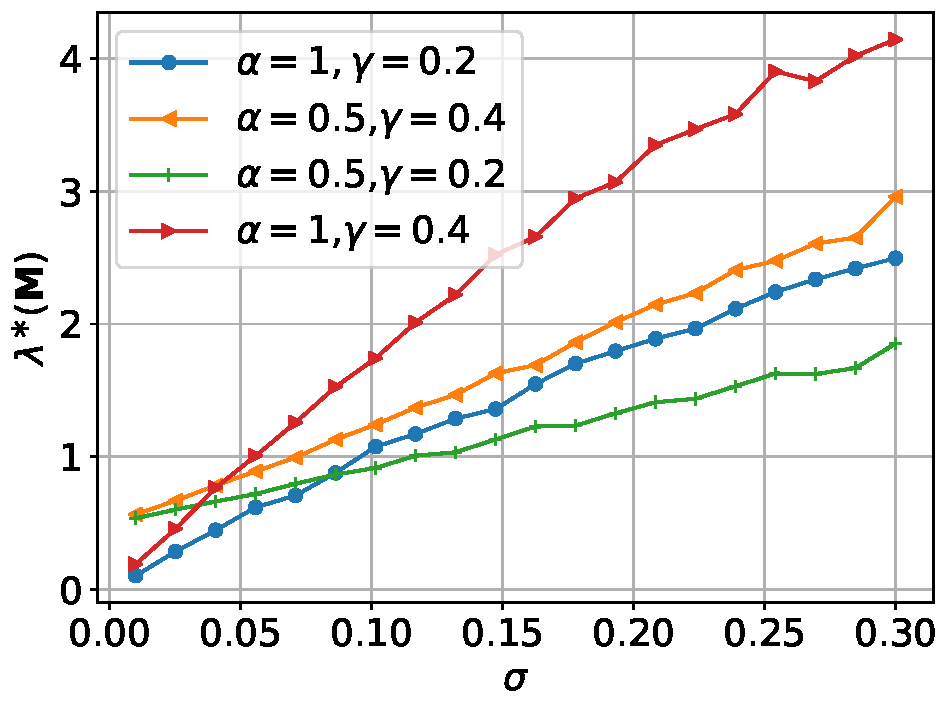
\includegraphics[width=0.6\columnwidth]{figures/converge/contraction_vs_variance_r1-crop.pdf}
  \caption{The largest singular value of $\bm{M}$ defined in \eqref{eq:matrix_m} versus variance of potential parameter $\bm{\theta}$. A value of each curve is the mean of $100$ graph realizations.}
  \label{fig:largest_singular}
\end{figure*}


In this section simulations on random graphs are carried out
to gain some insights on the $\alpha$-BP. The random graphs used here are generated
by the Erdos-R\'enyi (ER) model \cite{erdos1960}. In generating a graph by ER model, an edge between any two nodes is generated with probability $\gamma$, $\gamma \in (0,1)$.

Note that the MRF joint probability in \eqref{eq:mrf} can be reformulated into
\begin{equation}\label{eq:mrf_matrix_form}
  p(\bm{x}) \propto \exp\{-\bm{x}^{T}\bm{J}\bm{x} - \bm{b}^{T}\bm{x}\}, \bm{x} \in \bm{\Xx},
\end{equation}
with $\phi_{ts}(x_t, x_s) = e^{- 2 J_{t,s} x_t x_s}$ and $\phi_s(x_s) = e^{ - J_{s,s} x_s^2 - b_s  x_s}$. $\bm{J}$ here is the weighted adjacency matrix. In our experiments, we generate a random graph $\Gg = (\Vv, \Ee)$ with $\gamma$ by ER model and then associate potential factors to the graph. Specifically, factor $\phi_s(x_s)$ is associated to node $x_s$, $s \in \Vv$, and $\phi_{ts}$ to edge $(t, s) \in \Ee$. $J_{ts}$ is zero if these is no edge $(t, s)$.

For this set of experiments, we set $\Xx = \left\{ -1, 1 \right\}$ and $N=16$. To specify \eqref{eq:mrf_matrix_form}, the non-zero entries of $\bm{J}$ are sampled from a Gaussian distribution $\mathsf{N}(0, \sigma^2)$, i.e. $J_{ts} \sim \mathsf{N}(0, \sigma^2)$ if $J_{ts}\neq 0$. For entries of $\bm{b}$, we use $b_t \in \mathsf{N}(0, (\sigma/4)^2)$.
For each edge $(t,s) \in \Ee$, we set $\alpha_{ts}=\alpha$, i.e. the edges share a global value $\alpha$.

Figure~\ref{fig:largest_singular} illustrate how the largest singular value of $\bm{M}(\bm{\alpha}, \bm{\theta})$ as defined in \eqref{eq:matrix_m} changes when the standard deviation $\sigma$ of potential factors increases. The behavior is illustrated with different values of $\alpha$ and the edge probability $\gamma$. For each curve, a point on the curve is the mean of $100$ realizations of random graphs as described above. The curves of Figure~\ref{fig:largest_singular} show in general that a larger standard deviation of the potential factors of the graph edges makes it more difficult to fulfill the convergence condition in Theorem~\ref{thm:normd}. This is also the case when a graph is denser as we raise the edge probability $\gamma$ in generating random graphs, by comparing the green and orange curves. The comparison between green and blue curves indicates that the choice of $\alpha$ value in $\alpha$-BP also makes a difference, and its effect depends on the graph itself. Additionally, $\alpha$-BP with assignment $\alpha=0.5$ leads to flatter curves compared to standard BP ($\alpha=1$) and guarantees convergence for a larger range of $\sigma$, which corresponding a larger range of graphs.
How to tune $\alpha$ value to fulfill the condition of Theorem~\ref{thm:normd} depends not only on how dense ($\gamma$) the graph is, but also how potential factors spread out from each other.

\begin{figure*}[!t]
  \begin{subfigure}{0.5\textwidth}
    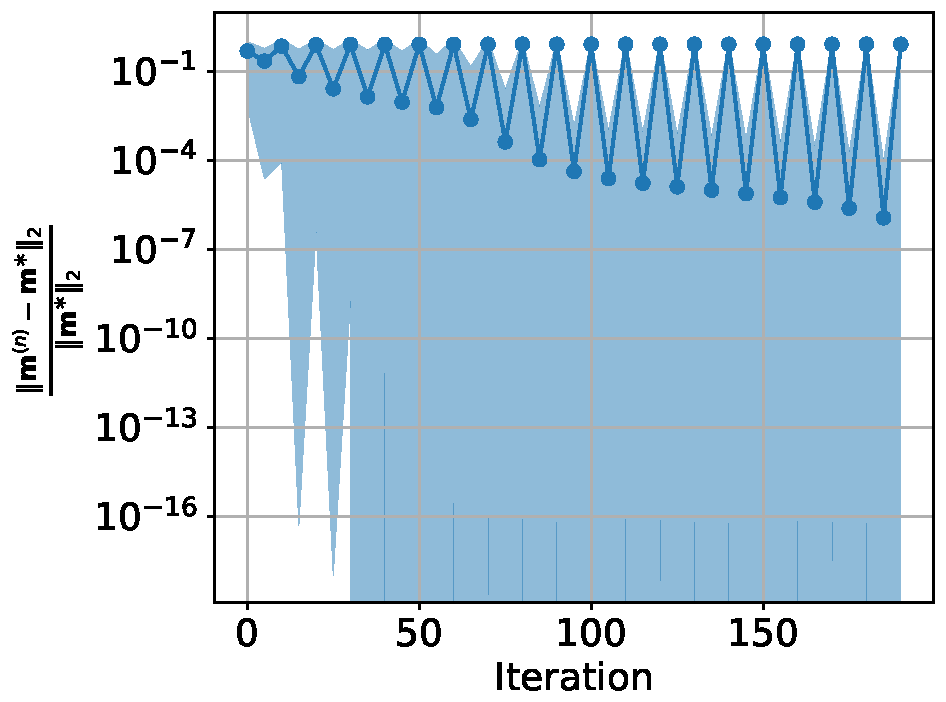
\includegraphics[width=1\columnwidth]
    {figures/converge/converge_erp0_4_alpha_1_stn_0_5_vs_filter_false_crop.pdf}
    \caption{}
    \label{fig:log-error-iter-diverse}
  \end{subfigure}
               %                the third figure
  \begin{subfigure}{0.5\textwidth}
    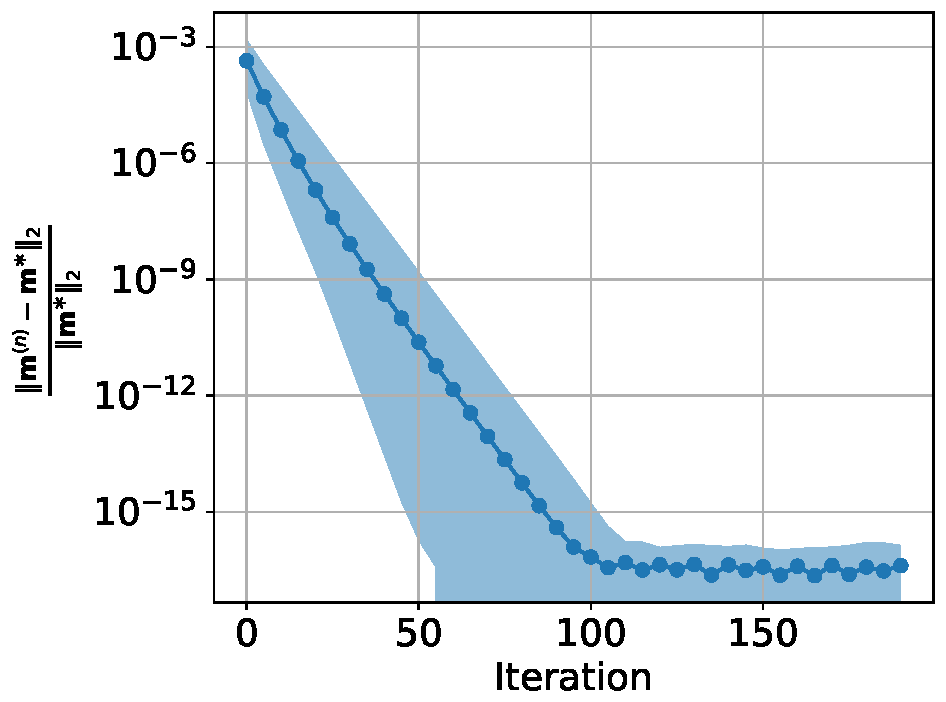
\includegraphics[width=1\columnwidth]{figures/converge/converge_erp0_2_alpha_0_5_stn_0_1_vs_filter_true-crop.pdf}
    \caption{}
    \label{fig:log-error-iter-converge}
  \end{subfigure}
  \caption{Numerical illustration of convergence, with normalized error ${\normd{\bm{m}^{(n)}-\bm{m}^{\ast}}}/{\normd{\bm{m}^{\ast}}}$ versus the number of iterations. Number of nodes $N=16$. (a) Parameter setting: $\gamma =0.4$, $\alpha = 1$ (equivalent to standard BP), $\sigma = 0.5$. (b) Parameter setting: $\gamma =0.2$, $\alpha = 0.5$, $\sigma = 0.1$.
    Blue region denotes the range from minimum to maximum of the normalized error of $100$ graph realizations, whereas the curve stands for mean error of the $100$ realized graphs. }
  \label{fig:convergence}
\end{figure*}



To illustrate our developed convergence condition for $\alpha$-BP, we also observe how messages in a graph changes along belief propagation iterations. To be specific, we run our $\alpha$-BP with $200$ iterations on a graph, after which the messages in the graph are denoted by $\bm{m}^{\ast}$. $\bm{m}^{\ast}$ can be the converged messages if $\alpha$-BP has converged within the $200$ iterations. Then we measure the quantity $\normd{\bm{m}^{(n)} - \bm{m}^{\ast}}/\normd{\bm{m}^{\ast}}$ during the iterations. In Figure~\ref{fig:log-error-iter-diverse}, we generate $100$ random graphs by ER model with parameter setting as $\gamma =0.4$, $\alpha = 1$\footnote{$\alpha=1$ in $\alpha$-BP corresponding to standard BP.}, $\sigma = 0.5$. By referring to the curves in Figure~\ref{fig:largest_singular}, it can be seen that this setting does not fulfill the condition in Theorem~\ref{thm:normd}. The log error changes versus iteration number $n$ for the $100$ graphs are shown in Figure~\ref{fig:log-error-iter-diverse}, in which the blue region indicates the range and the solid curve indicates the mean of the normalized errors. It is clear that Figure~\ref{fig:log-error-iter-diverse} does not show any sign of convergence within $200$ iterations.

\begin{figure*}[!t]
               %                the first figure
  \begin{subfigure}{0.5\textwidth}
    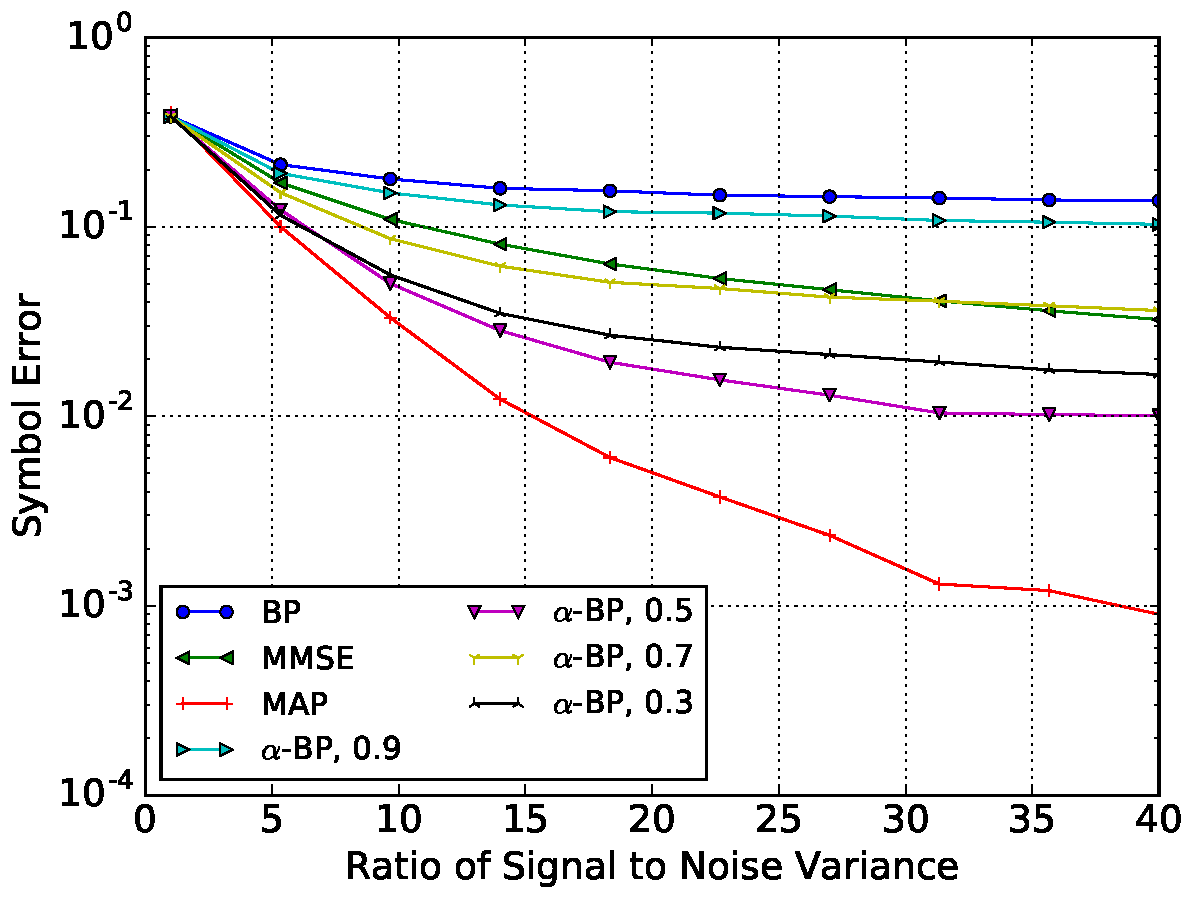
\includegraphics[width=1\columnwidth]{figures/alpha_compare_crop.pdf}
    \caption{}
    \label{fig:mimo_a}
  \end{subfigure}
  \begin{subfigure}{0.5\textwidth}
    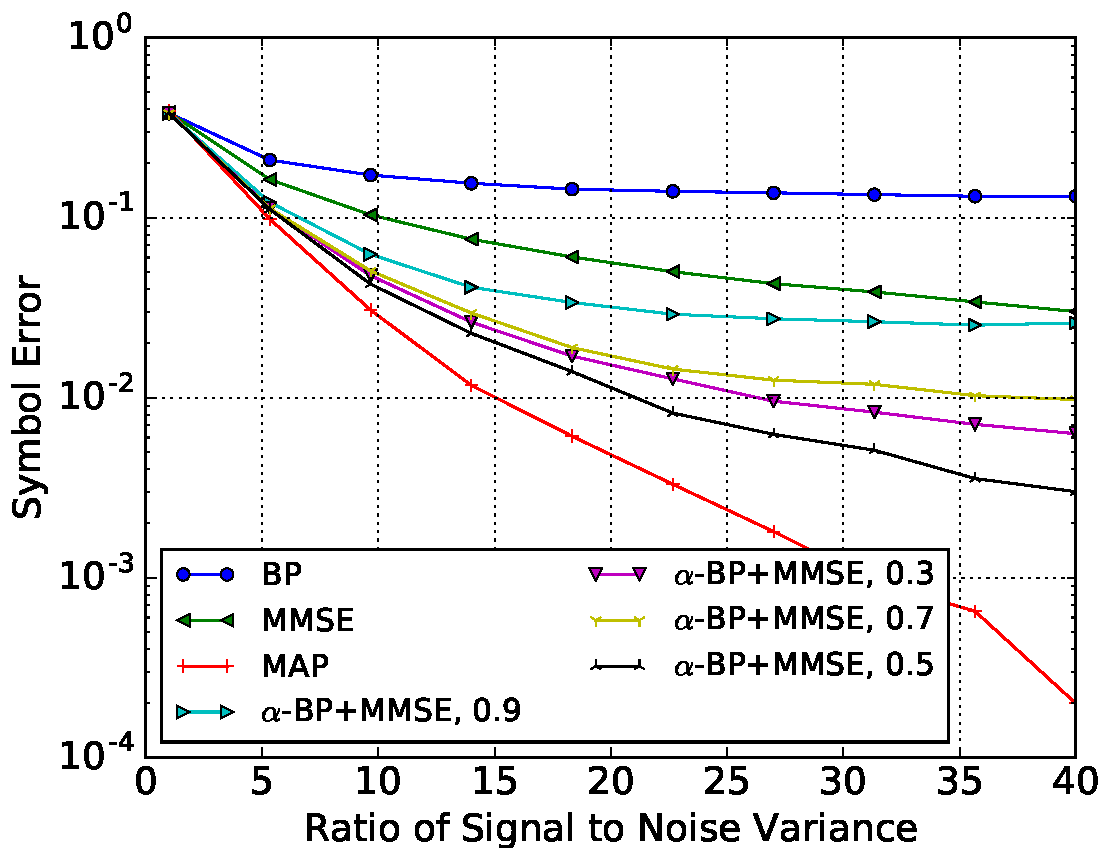
\includegraphics[width=1\columnwidth]{figures/prior_mmse_alpha_compare_crop.pdf}
    \caption{}
    \label{fig:mimo_b}
  \end{subfigure}
  \begin{subfigure}{0.5\textwidth}
    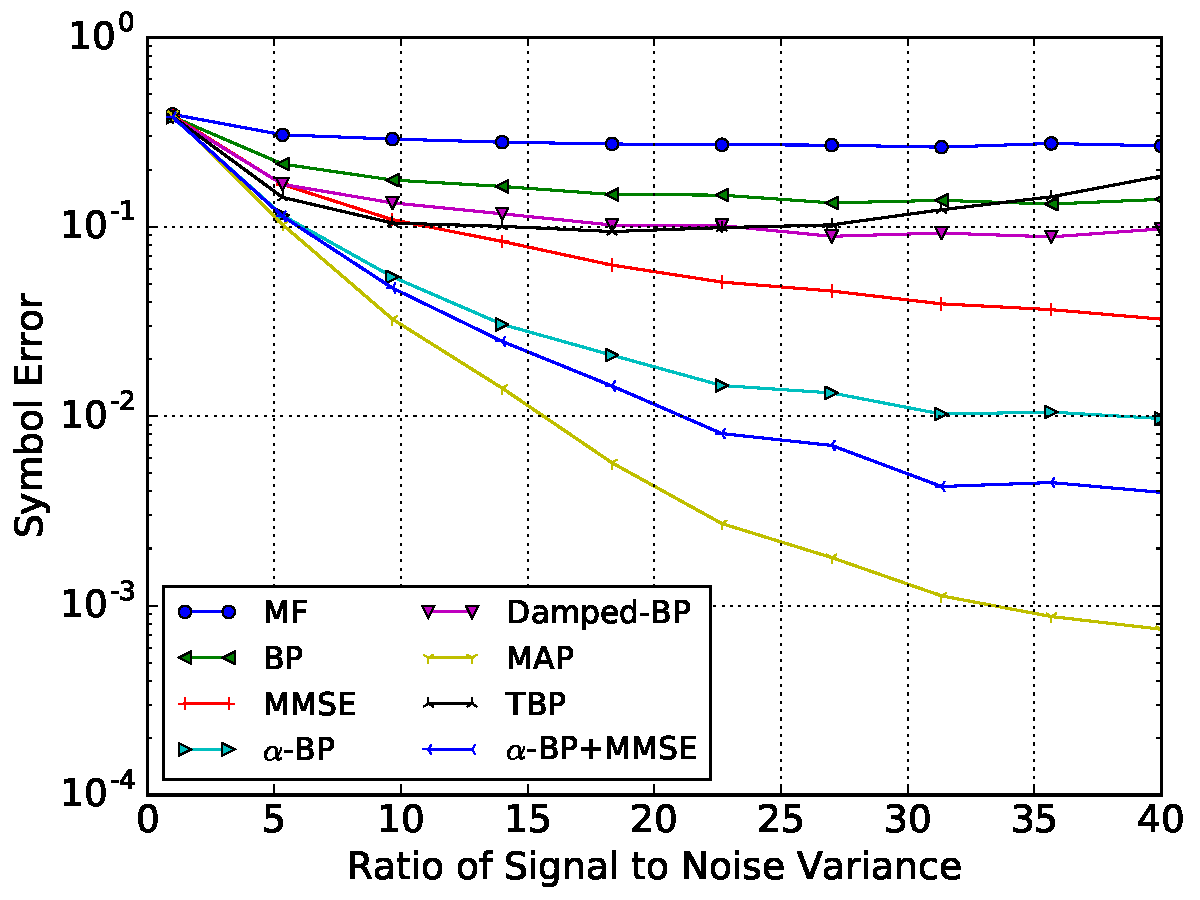
\includegraphics[width=1\columnwidth]{figures/tbp/mf_tbp_compare.pdf}
    \caption{}
    \label{fig:mimo_c}
  \end{subfigure}
  \caption{Numerical results of $\alpha$-BP: symbol error of MIMO detection.}
  \label{fig:mimo_detection}
\end{figure*}

We then carry out a set of experiments in Figure~\ref{fig:log-error-iter-converge} similar to our experiments in Figure~\ref{fig:log-error-iter-diverse}. The only difference lies in the graph generating process. Here we set the parameters to be $\gamma =0.2$, $\alpha = 0.5$, $\sigma = 0.1$. According to our curves in Figure~\ref{fig:largest_singular}, a graph generated with this parameter setting should fulfill the condition in Theorem~\ref{thm:normd}. Due to randomness of both graph generating by ER and potential factors, we regenerate a graph if the initial generated graph does not satisfy $\lambda^{\ast}(\bm{M})<1$. Therefore the $100$ graphs used in experiments for Figure~\ref{fig:log-error-iter-converge} all fulfill the Theorem~\ref{thm:normd}. The result in Figure~\ref{fig:log-error-iter-converge} is consistent with our analysis on the convergence of $\alpha$-BP.



\subsection{Complete Graph Case: Application to MIMO Detection}

In this section, we show the application of $\alpha$-BP to a multiple input multiple output (MIMO) detection problem. For a MIMO system, the observation $\bm{y}$ is a linear function of the channel $\bm{H}\in \RR^{N\times N}$ when the unknown signal $\bm{x}$ needs to be detected,
\begin{equation}\label{eq:linear-model}
  \bm{y} = \bm{H} \bm{x} + \bm{e}, \bm{x} \in \bm{\Xx},
\end{equation}
where $\bm{e}$ is  noise modeled as Gaussian noise $ \bm{e} \sim \mathsf{N}\left( \bm{0}, \sigma^2_{w} \bm{I} \right)$. Here $\bm{I}$ is \textit{unitary} matrix. In this case, the posterior of $\bm{x}$ can be written as:
\begin{align}\label{eq:true-posterior}
  p(\bm{x}|\bm{y}) &\propto e^{ - \frac{1}{2\sigma_w^2} \normd{\bm{Hx} - \bm{y}}^2 } \nonumber \\
                   & = e^{ - \frac{1}{2\sigma_w^2}\left[ \bm{x}^{T}\bm{H}^{T}\bm{H}\bm{x} - 2 \bm{y}^T\bm{H}\bm{x}  + \bm{y^T}\bm{y}  \right] }.
\end{align}
Denote $\bm{S} = \bm{H}^T\bm{H}$, $\bm{h}_i$ as the $i$-th column of $\bm{H}$, and
\begin{align}
  \phi_{i}(x_i) =& e^{- \frac{S_{i,i} x_i^2}{2 \sigma_w^2} + \frac{\langle {\bm{h}_i, \bm{y}}\rangle x_i}{\sigma_w^2} },\nonumber \\
  \phi_{ij}(x_i, x_j) =& e^{ -\frac{x_i S_{i,j} x_j}{\sigma_w^2} }.
\end{align}
Then it can be seen that \eqref{eq:true-posterior} is an instance of \eqref{eq:mrf}. We set $\Xx = \left\{ -1, 1 \right\}$, $N = 8$, and let $\bm{H}\in \RR^{8 \times 8}$ be sampled from a Gaussian distribution.

We test the application of $\alpha$-BP to the MIMO signal detection numerically. We run the $\alpha$-BP, without the prior trick (Subsection~\ref{subsec:remark}) in Figure~\ref{fig:mimo_a} and with the prior in Figure~\ref{fig:mimo_b} (legend ``$\alpha$-BP$+$MMSE'') as estimation of minimum mean square error (MMSE). The reference results of MMSE and maximum a posterior (MAP, exhausted search) are also reported under the same conditions. MMSE estimator depends on Gaussian posterior $\mathsf{N}(\hat{\bm{\mu}}, \hat{\bm{\Sigma}})$, where $\hat{\bm{\mu}} = (\bm{H}^{T}\bm{H} + \sigma_w^2 \bm{I})^{-1}\bm{H}^{T}\bm{y}$ and $\hat{\bm{\Sigma}} = (\bm{H}^{T}\bm{H} + \sigma_w^2 \bm{I})^{-1}\sigma_w$. Detection of MMSE carried out by $\argmin_{x_i\in \Xx}\abs{x_i-\hat{\mu}_i}$.% The prior belief used in ``$\alpha$-BP$+$MMSE'' is $\hat{p}(x_i)=\Nn(\hat{{\mu}}_i, \hat{\bm{\Sigma}}_{i,i})$.

Figure~\ref{fig:mimo_a} shows that BP even underperforms MMSE but $\alpha$-BP can outperform MMSE by assigning smaller value of $\alpha$.
Note that MMSE has a higher computation complexity since it requires the matrix inverse computation whose complexity is proportional to $N^3$. Therefore $\alpha$-BP is superior to MMSE both performance-wise and complexity-wise.  
                         %                          $\alpha$-BP does not have this problem and still can outperform MMSE. 
However, there is still a big gap between $\alpha$-BP (even for $\alpha=0.5$) and MAP. This gap can be decreased further by using the prior trick discussed in Subsection~\ref{subsec:remark}. Figure~\ref{fig:mimo_b} exemplifies this effects by using prior belief from MMSE, $\hat{p}_i(x_i)\propto \exp\{-(x_i-\hat{\mu}_i)^2/(2\hat{\bm{\Sigma}}_{i,i})\}$, by modifying the graph as shown in Figure~\ref{fig:factor-graph-with-prior}, which comes with legend "$\alpha$-BP$+$MMSE". It is shown that larger performance gain is observed when $\alpha$-BP runs with prior belief.

Additional, we also carry out the experiments where the proposed $\alpha$-BP is compared with mean field (legend 'MF'), BP with damping technique \cite{Pretti2005damping} (with legend 'Damped-BP'), and Tree-reweighted belief propagation \cite{wainwright2008graphical} (with legend 'TBP') in Figure~\ref{fig:mimo_c}. As expected, mean field method performs no better than BP. Damping technique improves BP's performance with a noticeable difference but still falls behind MMSE. The performance of tree-reweighted BP reaches that of MMSE in low ratio range of signal-to-noise variance but degenerates a lot in the high ratio range. The old message and potential factors are reweighted by the edge appearance probability in TBP to compute new messages. In TBP, the edge appearance probability is the probability that the edge exists in a randomly chosen spanning tree from all possible spanning trees of graph $\Gg$, which is usually expensive to compute.

\section{Summary}

In this chapter, we studied belief propagation in the way of $\alpha$-divergence minimization and proposed an alternative belief propagation method. The alternative method was connected and compared with the classic approximate iterative inference methods, namely mean filed, loopy belief propagation and tree-reweighted belief propagation. The connection and comparison were made with regard to both the high-level optimization objectives and the practical iterative update rules. All methods share a common interpretation, \textit{inference an optimization}, i.e., inference methods could be recovered from  optimization problems (free energy minimization or a divergence minimization). Although they started from different optimization cost functions, the derived iterative update rules share some similarities. The study enriches our insight into deterministic approximate inference approaches.

Given the wide application of the family of belief propagation methods, when the implementation of them can have guaranteed convergence is a fundamental question, which is of practical interest in general. This issue was addressed in the binary support case in this chapter via the method of contraction condition. The derived sufficient conditions for $\alpha$-BP gives us sufficient conditions about whether we can expect it to converge. The sufficient conditions allow us to check if $\alpha$-BP is guaranteed to converge without actually running the algorithm for a given problem.

Another essential question is about the error of deterministic approximate inference, compared with the exact answer. This problem is surely challenging. There is little work offering error-bounded methods in deterministic approximate inference family. Due to the lack of knowledge here, manual turning or trial-and-error is still not able to be avoided in practical system implementations. The development towards automated inference methods with at least less manual work is always an important direction in this track. 

\section{Relevant Literature}

Approximate inference is applicable to wide range of settings. The wide applications include but are not limited to imaging processing \cite{zhang2013denoise}, multi-input-multi-output (MIMO) signal detection in digital communication \cite{cespedes2014ep,jeon2015optimality}, inference on structured lattice \cite{10.2307/25651244}, and machine learning \cite{2018arXiv180607066M, Lin:2015:DLM:2969239.2969280, yoon2019inferenceGraph}. The empirical success of  belief propagation (BP) rules came much earlier than its theoretical examination, which dates back to $80$s in last century\cite{pearl1986b}.

As a result of the representation power of probabilistic graphical models, graphs with loops are inevitable in real-world problems. Before there was any justification, problems represented by graphs with loops simply employ BP as if there was no loop, i.e. loopy BP.  Although loopy BP is still a practical method to do inference approximately, its performance varies from case to case and its behavior is not well understood in general. A direct workaround is to propagate messages on a manipulated graph instead of the original graph. The representative methods of this family are junction tree (clique tree) method \cite[section~10]{koller2009pgm} and generalized belief propagation (GBP)\cite{yedida2005constucting}. Although they both cluster multiple nodes of the original graph into a node in a hyper-graph (clique tree or region graph) and propagate message in the new graph. Junction tree method provides an exact inference method while GBP is an approximate inference method. How to convert a general graph to a junction tree or region graph is not trivial, and the structure of the converted graph makes a significant difference in the inference performance. Additionally, the former's complexity relies on tree-width (the size of the largest clique minuses one), which means that there is not too much to gain by using junction tree compared to enumerating configurations in very dense graphs. For the latter, constructing a region graph itself is a challenging task and still needs further study.


Apart from the work of transforming the problem represented by a loopy graph into one of a hyper-graph, research is more active in approximate methods. Starting from the stationary point explanation of Bethe free energy in \cite{Yedidia:2000:GBP:3008751.3008848}, variants of BP have been derived to improve BP in a general graph. Fractional BP in \cite{Wiegerinck:2002:FBP:2968618.2968673} applies a correction coefficient to each factor and obtain a message passing rule similarly as minimization of Bethe free energy. 
Generalized BP in \cite{Yedidia:2000:GBP:3008751.3008848} propagates belief between different regions of a graph, and damping BP in \cite{Pretti2005damping} updates beliefs by combining old and new beliefs. \cite{wainwright2008graphical} relaxes a Bethe free energy into an upper bound of the partition function and the tree-reweighed BP is obtained. Technique such as damping is also explored to seek convergence of BP and its variants \cite{Pretti2005damping}.
Another track falls to the variational method framework, introduced by Opper and Winther \cite{Opper:2000:GPC:1121900.1121911} and Minka \cite{Minka:2001:EPA:647235.720257, Minka:2001:FAA:935427}, namely expectation propagation (EP). In EP, a simpler factorized distribution defined in exponential distribution family is used to approximate the original complex distribution, and an intuitive factor-wise refinement procedure is used to find such an approximate distribution. The method intuitively minimizes a localized Kullback-Leibler (KL) divergence. This is discussed further in \cite{divergence-measures-and-message-passing} and shows a unifying view of message passing algorithms. The following work, stochastic EP by \cite{yingzhen2015sep}, explores EP's variant method for applications to large datasets.

Due to the fundamental role of BP for probabilistic inference and related applications, research of seeking insight into BP performance and study on its convergence have been constantly carried out. \cite{weiss2000correctness} presents the convergence condition of BP in graphs containing a single loop. Work in \cite{heskes2004uniqueness} analyzes the Bethe free energy and offers sufficient conditions on the uniqueness of BP fixed point.
{Closely related to the content of this chapter, \cite{mooij2012sufficient-conditions} studies the sufficient conditions for BP convergence to a unique fixed point ($\alpha$-BP generalizes BP).}
\cite{nima2013stochasticBP} proposes a stochastic BP algorithm for high-dimensional discrete spaces and gives the convergence conditions of it. \cite{frederic2019fast} shows that BP can converge to global optima of Bethe energy when BP runs in Ising models that are ferromagnetic (neighboring nodes prefer to be aligned).
There are also works trying to give insight on variant methods of BP. Namely,
\cite{du2017convergenceBP, malioutov2006walk-sums} studies the convergence condition of Gaussian BP inference over distributed linear Gaussian models. \cite{roosta2008reweighed_sum_product} gives the convergence analysis of a reweighted BP algorithm, and offers the necessary and sufficient condition for subclasses of homogeneous graphical models with identical potentials.



%%% Local Variables:
%%% mode: latex
%%% TeX-master: "../../main"
%%% End:
